\clearpage
\section{Signal-candidate catalogue and conditional inpainting tests}
\label{app:signal-candidate-catalogue}

This appendix catalogues upward structures visible in the seven distinct
v4.2 upper-limit likelihood curves and tests whether replacing one such
structure by a smooth conditional background changes another mass point or a
combination containing the altered dataset.  The exercise is deliberately a
\emph{data-selected counterfactual diagnostic}.  It does not redefine the
accepted observed limit, provide a trials-corrected discovery probability, or
turn the conditional fixed-GP ensembles into coverage-calibrated bands.

\subsection{Operational catalogue from the seven limit curves}
\label{app:candidate-catalogue-rule}

The seven inputs are the three standalone curves, the three pair curves over
their genuine overlap intervals, and the all-three curve over 50--90~MeV.
The lower-order active-set tails drawn in the union panel are not counted a
second time.  The catalogue is constructed by the following reproducible
screen:

\begin{enumerate}
  \item retain a finite mass point when its observed 90\% \CLs{} upper limit
  lies strictly above the pointwise 97.5\% quantile of that curve's
  conditional fixed-state ensemble and its signed local excess is positive;
  \item merge adjacent one-MeV points into a curve-level island and represent
  the island by its minimum local $p_0$ point;
  \item merge islands across curves only when every pair of their
  one-resolution intervals overlaps (complete-link grouping); and
  \item choose the reference mass from the minimum-$p_0$ point in the
  highest-order supporting likelihood, preferring all-three, then a genuine
  pair, then standalone.
\end{enumerate}

The $\pm2.5\sigma_m$ inpainting windows are not used to merge features; doing
so would combine the physically distinct 80 and 90~MeV structures.  The
97.5\% quantile itself is only an operational graphical threshold: the
standalone and pairwise quantiles use 100 conditional draws and the
all-three quantile uses 300.  Their tail counts, local $p_0$ values, and
supporting combinations reuse data and conditional ensembles, so the largest
value in a feature is retained only as a descriptive catalogue entry.

\begin{landscape}
\begin{table}[H]
\centering
\small
\caption{Operational v4.2 signal-candidate catalogue.  ``Maximum $Z$'' is
the largest local asymptotic value among the data-sharing supporting scopes;
$R_{97.5}$ is the largest observed-limit to conditional-97.5\%-quantile
ratio in the feature.  Neither column is a globalized signal significance.}
\label{tab:v4p2-candidate-catalogue}
\begin{tabularx}{0.96\linewidth}{r r P{0.17\linewidth} r r Y}
\toprule
Reference & flagged span & standalone support & maximum $Z$ &
$R_{97.5}$ & comparison context \\
\midrule
21~MeV & 21 & 2015 & 2.516 & 1.149 &
singleton adjacent to the 2015 lower search edge \\
39~MeV & 39 & 2015 & 2.229 & 1.217 &
singleton coincident with the 2016 activation boundary \\
51~MeV & 49--52 & 2015, 2021 & 4.318 & 1.826 &
multi-dataset positional recurrence; 2021 is at its lower search edge and
2016 weakens the all-three result ($Z=2.381$) \\
65~MeV & 63--70 & 2015, 2016, 2021 & 4.657 & 1.827 &
broadest positional support; fixed-65 amplitudes vary among datasets and the
shared GP/profile refit shows reciprocal cross-response when the neighboring
80~MeV region is treated \\
80~MeV & 77--81 & 2021 & 2.873 & 1.440 &
chiefly supported by 2021; neighboring background-profile stress region in
the reciprocal inpainting/refit comparison \\
90~MeV & 86--93 & 2015, 2016 & 3.659 & 1.647 &
two-dataset recurrence, but exactly at the 2015 and 2015+2016 upper rail \\
117~MeV & 113--123 & 2016 & 3.277 & 1.483 &
substantial but single-dataset and broad \\
162~MeV & 159--164 & 2016 & 2.004 & 1.126 &
single-dataset secondary feature \\
\bottomrule
\end{tabularx}
\end{table}
\end{landscape}

The resulting eight entries form a finite catalogue of conditional-limit
excursion features and define the fixed comparison set below.  The tight
observed limits near 72--75~MeV record the neighboring deficit/background
structure; their proximity to the 65 and 80~MeV regions makes the moving-mask
response especially nonlocal in this interval.

\subsection{Native-histogram candidate-window inpainting protocol}
\label{app:candidate-inpainting-method}

Every catalogue mass is tested in every dataset active at that mass, giving
19 candidate--dataset interventions.  For each intervention, complete
post-rebin analysis bins are selected by centers inside the dataset-specific
continuous $m_c\pm2.5\sigma_m(m_c)$ interval.  Their corresponding native
0.05, 0.05, or 0.125~MeV bins are replaced; every native bin outside the
selected interval remains bitwise identical to the source histogram.  Thus
both the rebinned GP counts and the uncropped count-density integral used for
the $\eps^2$ conversion see the altered integer histogram.

The generating kernel constant and length scale are fixed to the reviewed
v4.2 state at $m_c$, but the GP posterior is reconditioned after excluding the
full $\pm2.5\sigma_m$ interval so that the removed feature cannot enter the
generating training sample.  The stochastic construction draws the complete
vector of excised analysis-bin intensities jointly from the count-space GP
posterior, using the same nonnegative \texttt{reject\_then\_clip} convention
as the conditional-band generator, and then draws Poisson analysis-bin
totals.  Smooth within-analysis-bin weights allocate each total
multinomially to native bins.  Three such draws are retained with matched
replicate labels.  A fourth, separate lane rounds the posterior mean
explicitly and uses largest-remainder native-bin allocation without a
Poisson draw.  That deterministic lane is a central reference and is not one
of the three replicates.

Each modified histogram is reused unchanged in the altered standalone
likelihood, every pair containing the altered dataset, and the all-active
combination.  Likelihoods excluding that dataset are exact no-change controls
by construction.  The inference step retains the accepted v4.2
$\pm2.25\sigma_m$ moving mask, physical density window, 12 optimizer
restarts, asymptotic \CLs{} calibration, and shared-$\eps^2$ combination.
Nearby catalogue anchors within 30~MeV are tested for every intervention; the
2021 removals at 65 and 80~MeV additionally use a one-MeV 55--95~MeV grid.

This pilot contains 76 native histograms, 564 optimized single-dataset fits,
and 2140 affected-scope likelihood results.  Every fit is finite.  One
deterministic 2021 fit initially selected a length-scale boundary; three
unchanged-card repeats found the same higher-likelihood interior family and
the maximum finite-LML solution was selected.  A subsequent branch audit
identified nine additional non-bound but substantially lower-LML states.
Three independent unchanged-card repeats per state found reproducible higher-
LML interior solutions for all nine; the maximum finite-LML solution was again
selected, with the other 554 single-fit rows unchanged.  Full attempt ledgers
are retained.  No final state is interpolated or on a kernel bound.  Fixed-
state reconstructions close in LML to $6.1\times10^{-6}$ or better, and all
outside-window native counts close bitwise.

For compact summaries an effect is labelled ``appreciable'' when
\begin{equation}
  \left|\log\!\left(\eps^2_{90,\mathrm{cf}}/
  \eps^2_{90,\mathrm{v4.2}}\right)\right|\geq\log(1.10)
  \quad\text{or}\quad |\Delta Z|\geq0.50 .
\end{equation}
This threshold is an engineering flag, not a hypothesis test.  All three
replicates and their median $[\min,\max]$ are retained; with $n=3$, no
standard error, recurrence probability, or coverage statement is assigned.

\begin{figure}[H]
\centering
\graphicorplaceholder{0.99\linewidth}{final_limit_projection_figs/v4p2_candidate_catalogue_20260807/candidate_inpainting_deltaZ_matrix.pdf}
\caption{Propagation into the all-active v4.2 likelihood.  Each cell is the
median local-$Z$ change across the three conditional posterior-predictive
inpainting replicates after removing the row feature from the dataset named
above the panel and evaluating the column feature.  Blank cells are
inapplicable or outside the predeclared 30~MeV neighborhood.  Diagonal
suppression is expected after replacing the selected excess; off-diagonal
cells expose moving-mask GP/profile cross-response.  Values are mechanism diagnostics,
not calibrated probabilities.}
\label{fig:v4p2-candidate-inpainting-matrix}
\end{figure}

The matrix shows that the fitted response extends beyond the replaced signal
window.  The strongest, clearest example is the reciprocal 65/80~MeV test in
2021.  At 80~MeV the fitted log-mass RBF length scale is about 0.304, whereas
$\log(80/65)=0.208$; the corresponding prior RBF correlation is approximately
$\exp[-\tfrac12(0.208/0.304)^2]=0.79$.  Thus the two windows are separated on
the signal-resolution scale while both remain within the nonlocal GP
correlation range and each can enter the other's moving-mask training sample.
The broad adjacent deficit/background structure can therefore transmit a
reciprocal change when the common profile is rerun.  This is a statement about
the refitting procedure rather than a physical dependence between the two
local features.

\begin{table}[H]
\centering
\small
\caption{Reciprocal 65/80~MeV result when the 2021 histogram is altered.  The
replicate columns give the median and full $[\min,\max]$ range of the three
conditional inpainting draws.  Ratios below one are tighter counterfactual
limits.  Here $r_{\rm UL}=\eps^2_{90,\rm cf}/\eps^2_{90,\rm v4.2}$.}
\label{tab:v4p2-reciprocal-65-80}
\begin{tabularx}{\linewidth}{llr P{0.17\linewidth} Y}
\toprule
Removal $\rightarrow$ test & likelihood & baseline $Z$ &
deterministic $(r_{\rm UL},\Delta Z)$ &
three-replicate median $[\min,\max]$: $r_{\rm UL}$; $\Delta Z$ \\
\midrule
65 $\rightarrow$ 80 & 2021 standalone & 2.641 & $(0.612,-1.540)$ &
$0.594\,[0.591,0.627]$; $-1.624\,[-1.635,-1.480]$ \\
65 $\rightarrow$ 80 & all three & 2.130 & $(0.632,-1.337)$ &
$0.616\,[0.613,0.646]$; $-1.409\,[-1.419,-1.283]$ \\
80 $\rightarrow$ 65 & 2021 standalone & 4.252 & $(0.708,-1.666)$ &
$0.569\,[0.538,0.706]$; $-2.478\,[-2.667,-1.688]$ \\
80 $\rightarrow$ 65 & all three & 3.993 & $(0.766,-1.275)$ &
$0.655\,[0.625,0.765]$; $-1.878\,[-2.020,-1.281]$ \\
\bottomrule
\end{tabularx}
\end{table}

\begin{figure}[H]
\centering
\graphicorplaceholder{0.99\linewidth}{final_limit_projection_figs/v4p2_candidate_catalogue_20260807/reciprocal_65_80_propagation.pdf}
\caption{Dense reciprocal 65/80~MeV response.  Black is the reviewed v4.2
observation.  Solid colored lines and bands are the median and full range of
the three inpainting replicates; dashed curves are the deterministic rounded-
mean lanes.  The upper row is 2021 standalone and the lower row is the
all-active union likelihood (all three datasets through 90~MeV and
2016+2021 above it).  Altering either window and rerunning the shared
GP/profile changes both fitted curves and redistributes local excess and limit
structure across the 55--95~MeV interval.  This measures a profile response,
not an interaction between physical signals.}
\label{fig:v4p2-reciprocal-65-80}
\end{figure}

The earlier 65~MeV GP-mean replacement identified a procedural sensitivity,
and the reverse test shows that this sensitivity is reciprocal under the same
shared fit.  Neither direction is assigned a causal interpretation.  Each
excision changes training data used by the nonlocal profile, and the broad
72--75~MeV deficit/background structure can transmit that change across the
interval.  We therefore describe a model-mediated cross-response while
retaining the 65 and 80~MeV regions as distinct local features.  Neither
excision is substituted for the reviewed observation.

\subsection{Position of the 65 MeV excess across datasets}
\label{app:m065-positional-overlay}

\begin{figure}[H]
\centering
\graphicorplaceholder{0.93\linewidth}{final_limit_projection_figs/v4p2_candidate_catalogue_20260807/m065_standalone_z_positional_overlay.pdf}
\caption{Standalone local-$Z$ scans near 65~MeV, overlaid without smoothing
or interpolation.  The maxima are at 64, 68, and 65~MeV for 2015, 2016, and
2021.  Relative to 65~MeV these are $-0.30$, $+1.13$, and $0$ times the
dataset-specific resolution.}
\label{fig:v4p2-m065-z-overlay}
\end{figure}

\begin{figure}[H]
\centering
\graphicorplaceholder{0.93\linewidth}{final_limit_projection_figs/v4p2_candidate_catalogue_20260807/m065_standardized_residual_positional_overlay.pdf}
\caption{The exact fixed-state 65~MeV profiled Pearson-residual inputs on the
common coordinate $(m-65~\mathrm{MeV})/\sigma_m(65)$, again with no
interpolation.  The profiles support resolution-scale positional comparison,
but their bins are correlated likelihood diagnostics rather than independent
bin significances.}
\label{fig:v4p2-m065-residual-overlay}
\end{figure}

The peak positions are compatible with one resolution-scale location, but
the amplitudes are less coherent.  At exactly 65~MeV the standalone local
$Z$ values are 2.395, 0.595, and 4.252.  A Gaussian common-strength
compatibility calculation gives approximately $Q=8.16$ for two degrees of
freedom ($p\simeq0.017$), driven by the weak/down-pulling 2016 estimate.
Thus the overlay supports positional recurrence, not a common signal-yield
claim.

\subsection{Conditional 2021 10\% SIMP/TM kinematic atlas}
\label{app:m065-kinematic-atlas}

The exact observed-limit histogram was built from the v16 prompt-target-
constrained, $p_{\rm sum}>2.8$ production.  Its full event-level directory is
not locally mounted.  The available full-statistics kinematic source is a
different frozen v11 SIMP/TM atlas with 1186 input files and 293,397,563
selected rows scanned.  The following plots are therefore conditional
selected-row mechanism diagnostics; they are not the kinematics of the exact
events entering the observed v4.2 limit, a fitted candidate yield, or an
independent significance.

The central interval is the physical 2021
$65\pm2.5\sigma_m=[59.696,70.304]$~MeV window.  The nominal two sidebands span
2.5--4.0$\sigma_m$ and are scaled by mass width.  Stopping at
4$\sigma_m$ keeps the right sideband below the 80~MeV candidate's own
$\pm2.5\sigma_m$ interval.  Four stored kinematic surfaces are available:
pair momentum sum, reconstructed vertex $z$, vertex-projection significance,
and the minimum-track $|y_0|$ proxy.

\begin{figure}[H]
\centering
\graphicorplaceholder{0.96\linewidth}{final_limit_projection_figs/v4p2_candidate_catalogue_20260807/candidate65_window_sideband_simp_low_mass_y0.pdf}
\caption{Central and width-scaled sideband kinematic distributions in the
stricter v11 SIMP low-mass, topology-dependent minimum-$y_0$ lane.  Their
close agreement corresponds to an aggregate local-subtraction residual of
$-4.5\pm31.8$ selected rows.}
\label{fig:v4p2-m065-kinematics-lowmass}
\end{figure}

\begin{figure}[H]
\centering
\graphicorplaceholder{0.96\linewidth}{final_limit_projection_figs/v4p2_candidate_catalogue_20260807/candidate65_window_sideband_tm_high_mass_y0.pdf}
\caption{The same selected-row comparison in the v11 TM/SIMP high-mass
minimum-$y_0$ lane.  The aggregate residual is $+336.4\pm122.0$ rows, but its
topology and sideband dependence prevent a signal interpretation.}
\label{fig:v4p2-m065-kinematics-highmass}
\end{figure}

\begin{figure}[H]
\centering
\graphicorplaceholder{0.96\linewidth}{final_limit_projection_figs/v4p2_candidate_catalogue_20260807/candidate65_topology_residual.pdf}
\caption{Topology decomposition of the local sideband subtraction.  The
high-mass-lane residual is concentrated in L2L2
($329.5\pm107.4$ rows), while the stricter low-mass lane has no stable
aggregate residual.  The very large broad-atlas residual has incompatible
topology signs and is a selection/mass-correlation warning.}
\label{fig:v4p2-m065-kinematics-topology}
\end{figure}

\begin{figure}[H]
\centering
\graphicorplaceholder{0.96\linewidth}{final_limit_projection_figs/v4p2_candidate_catalogue_20260807/candidate65_sideband_choice_stress.pdf}
\caption{Dependence of the locally subtracted selected-row count on the outer
sideband edge.  The residual rises as the sideband is widened; the gray region
marks choices whose sideband overlaps the 80~MeV $\pm2.5\sigma_m$ window.
This behavior demonstrates the aggregate residual's sensitivity to sideband
choice and motivates the exact-v16 chord comparisons below.}
\label{fig:v4p2-m065-kinematics-sidebands}
\end{figure}

The available v11 atlas therefore supplies a concrete
instrumental/selection hypothesis---especially the L2L2 concentration---and
motivates the sample-matched exact-v16 comparisons added below.  A
candidate-level kinematic inference additionally requires unique-event
semantics, category-specific signal response, and a correlation-preserving
background treatment.

\subsection{Descriptive synthesis and follow-up}
\label{app:candidate-assessment}

The 65~MeV region remains the most informative interior follow-up because it
has the broadest positional recurrence and largest all-three local excess.
The 51~MeV feature has exact-position recurrence in 2015 and 2021 while
touching the 2021 lower search rail; the 90~MeV feature recurs in 2015 and
2016 at their upper overlap rail; and 117~MeV is a broad 2016-only structure.
The 80~MeV region is retained as its own local feature and as a neighboring
background-profile stress region.  Reciprocal inpainting/refit response near
65 and 80~MeV is model-mediated through the shared nonlocal GP/profile and
adjacent deficit structure; it is not a claim that one feature physically
depends on the other.

The corresponding follow-up program is a predeclared joint 65+80 union
excision, denser unchanged-card optimizer-repeat review of the affected
interval, full-procedure signal-injection and background-only coverage studies
with the same moving-mask refit, scan-wise calibration, and an event-identified
v16 kinematic comparison.  The present appendix supplies the catalogue and
mechanism screen used to define those tests.

\subsection{Exact-v16 selected-row morphology diagnostics}
\label{app:v4p3-exact-v16-diagnostics}

The preceding kinematic atlas used a v11 SIMP/TM production because the exact
event-level source of the v4.2 observed-limit histogram was not then locally
available.  A new v16 diagnostic production now supplies the unchanged
prompt-target-constrained, $p_{\rm sum}>2.8$ baseline together with exhaustive
topology and stored-trigger partitions and four mass-versus-control
histograms.  This closes the earlier \emph{histogram-level} sample mismatch:
the 2000-, 4000-, and 8000-bin invariant-mass histograms, including their
axes, are bitwise identical to the frozen v4.2 2021 input and each contains
141,590,915 selected rows.  Unique physical-event counting remains outside
this histogram-level closure because the parser did not identify a stable
run/event key.

\begin{table}[H]
\centering
\small
\caption{Release-level continuity checks for the exact-v16 diagnostic
product.  ``Exact'' refers to histogram arrays and axes, not to an
independently frozen event-file list or unique-event identity.}
\label{tab:v4p3-v16-provenance}
\begin{tabularx}{0.96\linewidth}{P{0.31\linewidth} P{0.24\linewidth} Y}
\toprule
gate & result & qualification \\
\midrule
canonical baseline, 2000/4000/8000 bins & bitwise exact; 141,590,915 rows &
matches the frozen v4.2 spectrum at all three binnings \\
six topology categories & exact binwise partition closure &
includes the 25.6\% \texttt{topology\_other} category \\
four stored-trigger flag categories & exact binwise partition closure &
the ``neither'' category is empty; categories are exclusive stored-flag combinations \\
1-MeV mass-retention sidecar & 11 selections $\times$ 260 bins exact &
all values reproduce aggregations of the 8000-bin ROOT histograms \\
input-file provenance & 1189 unique paths; list hash recorded &
status remains \texttt{list-hash-unfrozen} \\
row semantics & selected candidate rows &
unique-event mapping and inter-row correlations are unavailable \\
\bottomrule
\end{tabularx}
\end{table}

The four controls are pair momentum sum, vertex-projection significance,
the minimum-track $|y_0|$ proxy, and the stored electron-track 3D-hit count.
The last quantity is not the N2D-hit variable used in earlier selection
studies, and vertex-projection significance is not reconstructed vertex
$z$.  No new vertex-$\chi^2$, momentum, opening-angle, or $y_0$ cut is made.
The control-axis overflows are retained in the ledger; the displayed 2D
domains omit 395 vertex-significance rows and 7368 $y_0$ rows, while the
mass axis omits 82,471 rows below 40~MeV and 256,936 above 300~MeV.

\subsubsection{Sideband-trained conditional-composition GPR}
\label{app:v4p3-composition-gpr-method}

The available histograms do not support an event-level two-dimensional
signal likelihood.  In particular, there is no signal template in the second
coordinate, no category-specific efficiency or mass-resolution model, and no
validated factorization of selected rows into independent events.  The useful
part of the true-muonium 2D-GPR construction is therefore adapted only as a
background-morphology diagnostic: a target-masked smooth surface is fit to
the mass dependence of the conditional control composition.

For mass bin $i$ and one of $J$ mutually represented control groups, let
$N_{ij}$ be the selected-row count and $N_i=\sum_jN_{ij}$.  The fitted
coordinates are the Jeffreys-regularized centered log ratios
\begin{equation}
 p_{ij}=\frac{N_{ij}+1/2}{N_i+J/2},\qquad
 y_{ij}=\log p_{ij}-\frac{1}{J}\sum_{k=1}^{J}\log p_{ik}.
 \label{eq:v4p3-clr-gpr}
\end{equation}
Independent mass-axis RBF predictors for the $y_{ij}$ coordinates are
coupled again by the inverse centered-log-ratio transform, so every predicted
composition sums to one.  This conditions on the observed mass-bin total and
tests morphology only; it neither estimates the total background under a
candidate nor assigns a signal yield.

The primary card uses 0.5-MeV mass bins over 40--160~MeV and eight contiguous
control groups whose boundaries are frozen from candidate-masked sideband
rows.  The eight stored 3D-hit bins, six exhaustive topology categories, and
three nonempty trigger categories remain discrete.  The union of the fixed
$65\pm2.5\sigma_m$ and $80\pm2.5\sigma_m$ stripes is excluded from both
kernel choice and training to protect the interpolation against reciprocal
model-mediated cross-response.  Such cross-response can arise through the
common nonlocal GP/background profile and adjacent deficit/background
structure.  It is assigned to the shared fitting procedure rather than to
physical causation, shared events, or intrinsic dependence between the
features.  For each surface the RBF length
and
standardized nugget are chosen from
\begin{equation}
 \ell_m\in\{2,4,8,12,20,35\}\ \mathrm{MeV},\qquad
 \eta\in\{10^{-4},10^{-3},10^{-2},5\times10^{-2}\},
\end{equation}
using the median centered-log-ratio residual in five same-rule held-out fake
gaps at 50, 100, 115, 130, and 145~MeV.  None of those scores is converted to
a $p$-value or significance.  Deterministic checks repeat the procedure at
0.125, 0.25, 0.5, and 1.0~MeV mass binning, with 6, 8, 10, and 12 continuous
control groups, and with single-target rather than union masks.  No
pseudoexperiment, expected band, or coverage claim is introduced in v4.3.

\begin{figure}[H]
\centering
\graphicorplaceholder{0.98\linewidth}{final_limit_projection_figs/v4p3_2021_10pct_exact_v16_diagnostics_20260810/partition_composition_gpr.pdf}
\caption{Exact-v16 topology and stored-trigger compositions aggregated over
the 65 and 80~MeV target stripes.  Black bars are observed selected-row
fractions and orange bars are the jointly masked, sideband-trained
conditional-composition GPR predictions.  The exact partition closures are a
data-integrity result.  The displayed interpolation is a correlated
histogram-level morphology diagnostic, not a category signal fit.}
\label{fig:v4p3-partition-composition}
\end{figure}

\subsubsection{Fixed-window controls and mass-surface residuals}
\label{app:v4p3-control-results}

The exact parser windows contain 16,361,818 rows at 65~MeV and 20,984,092 rows
at 80~MeV.  Subtracting the combined adjacent sidebands after the prescribed
$5/3$ width scaling gives $+1,039,881$ and $+557,880$ rows, respectively.
Those large values are spectrum-curvature diagnostics: 65~MeV lies on the
rising shoulder of a distribution whose broad maximum is near 77.5~MeV.
They are not fitted candidate yields.  After normalizing the central and
combined-sideband control distributions separately and applying the primary
control grouping, the total-variation distances span only 0.12--1.02\% across
the four saved variables.  Lower and
upper sidebands move in opposite directions for several controls, confirming
that a one-number sideband subtraction is mass sculpted.

\begin{figure}[H]
\centering
\graphicorplaceholder{0.98\linewidth}{final_limit_projection_figs/v4p3_2021_10pct_exact_v16_diagnostics_20260810/central_sideband_controls.pdf}
\caption{Normalized exact-v16 control distributions in each central stripe
and its lower, upper, and combined adjacent sidebands.  Each curve is
normalized independently to expose shape rather than the rapidly changing
mass yield.  The visible lower-to-upper evolution motivates the
mass-conditioned GPR; none of these differences is a fitted signal
component.}
\label{fig:v4p3-central-sideband-controls}
\end{figure}

\begin{figure}[H]
\centering
\graphicorplaceholder{0.98\linewidth}{final_limit_projection_figs/v4p3_2021_10pct_exact_v16_diagnostics_20260810/conditional_residual_atlas.pdf}
\caption{Observed minus GPR-predicted conditional composition in the 65 and
80~MeV target stripes for the four mass--control surfaces and the topology and
trigger partitions.  Colors are percentage-point composition residuals, not
Poisson pulls.  All panels reuse the same selected rows and must not be
combined as independent tests.}
\label{fig:v4p3-conditional-residual-atlas}
\end{figure}

The parent v4.2 deterministic inpainting supplies a useful scale for the
dilution of any local component.  In its complete analysis-bin windows,
$(N_{\rm data}-N_{\rm GP\ mean})/N_{\rm data}$ is 0.2605\% at 65~MeV and
0.1460\% at 80~MeV.  These are conditional mean-fill differences, not signal
purities.  The parent counterfactual changes each complete window total by
less than 0.3\%, which illustrates the severe dilution scale but does not
identify the remaining rows as background.  Sub-percent composition changes
therefore cannot by themselves distinguish a dilute prompt signal from
ordinary mass dependence or reconstruction effects.

\begin{figure}[H]
\centering
\graphicorplaceholder{0.98\linewidth}{final_limit_projection_figs/v4p3_2021_10pct_exact_v16_diagnostics_20260810/effect_size_robustness_summary.pdf}
\caption{Conditional-composition effect sizes and deterministic closure
context at 65 and 80~MeV.  The upper panels show the primary maximum
composition shift and its ratio to the median fake-gap CLR residual; the
ratio is not a $p$-value.  In the lower panels, filled markers show the
primary union-masked card and line segments span the mass-binning variants.
The ranges are model-robustness envelopes, not confidence intervals.  Parent
v4.2 mean-fill fractions are included only as dilution references.}
\label{fig:v4p3-effect-size-summary}
\end{figure}

The 65~MeV stripe has modest, repeatable changes in some momentum-sum,
topology, and high-$|y_0|$ fractions, while the trigger composition is nearly
unchanged.  The detailed vertex-significance and 3D-hit-bin directions are
less stable under reasonable binning and grouping choices.  At 80~MeV the
effects are generally smaller and their leading bins or signs change more
often across the deterministic variations.  Because each comparison reuses
the same selected rows and conditions on the mass-bin total, differences
across variables or regions are correlated descriptors rather than separate
tests.  In particular, the joint mask does not convert shared-model
cross-response into a statement about the physical relation between the
65 and 80~MeV features.

Thus the exact-v16 product removes the earlier histogram-level sample
mismatch and provides a controlled view of saved-variable morphology.  The
histograms alone do not furnish an event-level signal template, fitted yield,
or calibrated local or global significance.  Event-identified run/time
splits, category-specific signal simulation and response, and
correlation-preserving inference would be required for those quantities.

\subsection{Exact-v16 candidate-region variable comparisons}
\label{app:v4p3-candidate-region-comparisons}

The exact-v16 mass--control surfaces permit one common regional comparison at
six catalogue anchors inside their support: 51, 65, 80, 90, 117, and
162~MeV.  The 21 and 39~MeV entries are omitted solely because these surfaces
begin at 40~MeV; the omission is a surface-support choice and not an ordering
of the catalogue features.  The displayed quantities are overlap-weighted
histogram approximations to normalized selected-row shapes and category
fractions.  They do not define a fitted signal yield, significance, or limit.

For anchor $m_0$ and the frozen resolution $\sigma_m(m_0)$, define the
half-open lower, central, and upper regions
\begin{equation}
\begin{aligned}
 \mathcal{L}(m_0) &=[m_0-4\sigma_m,\,m_0-2.5\sigma_m), \\
 \mathcal{C}(m_0) &=[m_0-2.5\sigma_m,\,m_0+2.5\sigma_m), \\
 \mathcal{U}(m_0) &=[m_0+2.5\sigma_m,\,m_0+4\sigma_m).
\end{aligned}
\label{eq:v4p3-candidate-region-windows}
\end{equation}
For native 0.125-MeV mass bin $i$ with edges $[a_i,b_i)$, its contribution
to region $R$ is weighted by
\begin{equation}
 w_{iR}=\frac{\left|[a_i,b_i)\cap R\right|}{b_i-a_i}.
 \label{eq:v4p3-region-overlap-weight}
\end{equation}
Thus a region total or control-bin count is a fractional edge-overlap sum,
$N_{Rj}=\sum_i w_{iR}N_{ij}$, rather than a native-bin-center selection.
Every regional distribution is normalized independently,
$p_{Rj}=N_{Rj}/\sum_kN_{Rk}$, so the comparison concerns shape rather than
the rapidly varying mass yield.  Because the two sidebands have equal width,
their symmetric first-order local reference is the composition chord
\begin{equation}
 p_{{\rm chord},j}=\frac{p_{\mathcal{L},j}+p_{\mathcal{U},j}}{2},\qquad
 \Delta_j=100\left(p_{\mathcal{C},j}-p_{{\rm chord},j}\right),\qquad
 \mathrm{TV}=\frac{1}{2}\sum_j
 \left|p_{\mathcal{C},j}-p_{{\rm chord},j}\right|.
 \label{eq:v4p3-region-comparison-statistics}
\end{equation}
Here $\Delta_j$ is a percentage-point shape residual and TV is a descriptive
distance.  Neither is a pull or calibrated test statistic.

For continuous controls, display groups are frozen from rows outside the
union of all six fractional central regions and then reused without retuning
at individual anchors.  This prevents any one catalogue window from setting
the display-bin edges.  The six surfaces reuse selected rows, so comparisons
across variables are correlated descriptions of the same production.

The 65 and 80~MeV central windows are disjoint: the first ends at
70.304~MeV and the second begins at 74.280~MeV.  Their adjacent sidebands
overlap from 70.849 to 73.487~MeV and therefore sample part of the same
neighboring deficit/background interval.  The 80 and 90~MeV central windows
overlap from 83.950 to 85.720~MeV, and their adjacent sidebands also cross
into the neighboring central interval.  The anchor panels are consequently
regional views, not a partition into disjoint selected-row samples.

For validation at 65 and 80~MeV, the baseline-closed momentum-sum,
electron-hit, topology, and trigger surfaces have overlap-weighted central
totals of 16,361,498 and 20,983,869 rows, compared with the parser-exact
totals of 16,361,818 and 20,984,092.  The corresponding overlap-weighted
combined-sideband totals are 9,193,205 and 12,256,152 rows, compared with
parser-exact values of 9,193,162 and 12,255,727.  These few-$10^{-5}$ relative
differences are the expected consequence of applying continuous window edges
to saved mass histograms.  The vertex-significance and minimum-$|y_0|$
surfaces retain their separately recorded control-axis flow qualifications;
their per-surface totals are given in the machine-readable ledger.

\subsubsection{Saved control-variable shapes}
\label{app:v4p3-candidate-region-continuous}

Figures~\ref{fig:v4p3-candidate-region-psum}--
\ref{fig:v4p3-candidate-region-electron-n3d-hits} apply the same region
geometry and grouping ledger to three continuous controls and the stored
discrete electron 3D-hit count.  Lower and upper sidebands remain separate,
while the chord supplies a symmetric local reference.

\begin{figure}[H]
\centering
\graphicorplaceholder{0.98\linewidth}{final_limit_projection_figs/v4p3_candidate_region_variable_comparisons_20260811/candidate_region_psum.pdf}
\caption{Overlap-weighted, normalized pair-momentum-sum distributions in the
central, lower-sideband, and upper-sideband regions at 51, 65, 80, 90, 117,
and 162~MeV, with the equal-sideband chord as the local shape reference.}
\label{fig:v4p3-candidate-region-psum}
\end{figure}

\begin{figure}[H]
\centering
\graphicorplaceholder{0.98\linewidth}{final_limit_projection_figs/v4p3_candidate_region_variable_comparisons_20260811/candidate_region_vtx_proj_sig.pdf}
\caption{Overlap-weighted, normalized vertex-projection-significance
distributions and chord references in the same six regions.  Vertex-
projection significance is not reconstructed vertex $z$.}
\label{fig:v4p3-candidate-region-vtx-proj-sig}
\end{figure}

\begin{figure}[H]
\centering
\graphicorplaceholder{0.98\linewidth}{final_limit_projection_figs/v4p3_candidate_region_variable_comparisons_20260811/candidate_region_min_y0.pdf}
\caption{Overlap-weighted, normalized minimum-track $|y_0|$-proxy
distributions and chord references in the same six regions.  Display groups
are frozen with the union of all six central regions masked.}
\label{fig:v4p3-candidate-region-min-y0}
\end{figure}

\begin{figure}[H]
\centering
\graphicorplaceholder{0.98\linewidth}{final_limit_projection_figs/v4p3_candidate_region_variable_comparisons_20260811/candidate_region_electron_n3d_hits.pdf}
\caption{Overlap-weighted, normalized stored electron-track 3D-hit-count
distributions and chord references in the same six regions.  This quantity is
distinct from the N2D-hit variable used in earlier selection studies.}
\label{fig:v4p3-candidate-region-electron-n3d-hits}
\end{figure}

\subsubsection{Exhaustive category comparisons}
\label{app:v4p3-candidate-region-categories}

The topology panels use the six exhaustive saved categories, including
\texttt{topology\_other}.  The stored-trigger panels use the three populated
flag categories; they summarize stored flag combinations rather than
independent trigger samples.  Exact partition closure is inherited from the
release-level checks in Table~\ref{tab:v4p3-v16-provenance}.

\begin{figure}[H]
\centering
\graphicorplaceholder{0.98\linewidth}{final_limit_projection_figs/v4p3_candidate_region_variable_comparisons_20260811/candidate_region_topology.pdf}
\caption{Overlap-weighted topology fractions and chord references in the
central and adjacent-sideband regions at all six supported anchors.  Each
regional category vector is normalized to unity.}
\label{fig:v4p3-candidate-region-topology}
\end{figure}

\begin{figure}[H]
\centering
\graphicorplaceholder{0.98\linewidth}{final_limit_projection_figs/v4p3_candidate_region_variable_comparisons_20260811/candidate_region_trigger.pdf}
\caption{Overlap-weighted stored-trigger-category fractions and chord
references in the same six regions.  Each regional category vector is
normalized to unity.}
\label{fig:v4p3-candidate-region-trigger}
\end{figure}

\begin{figure}[H]
\centering
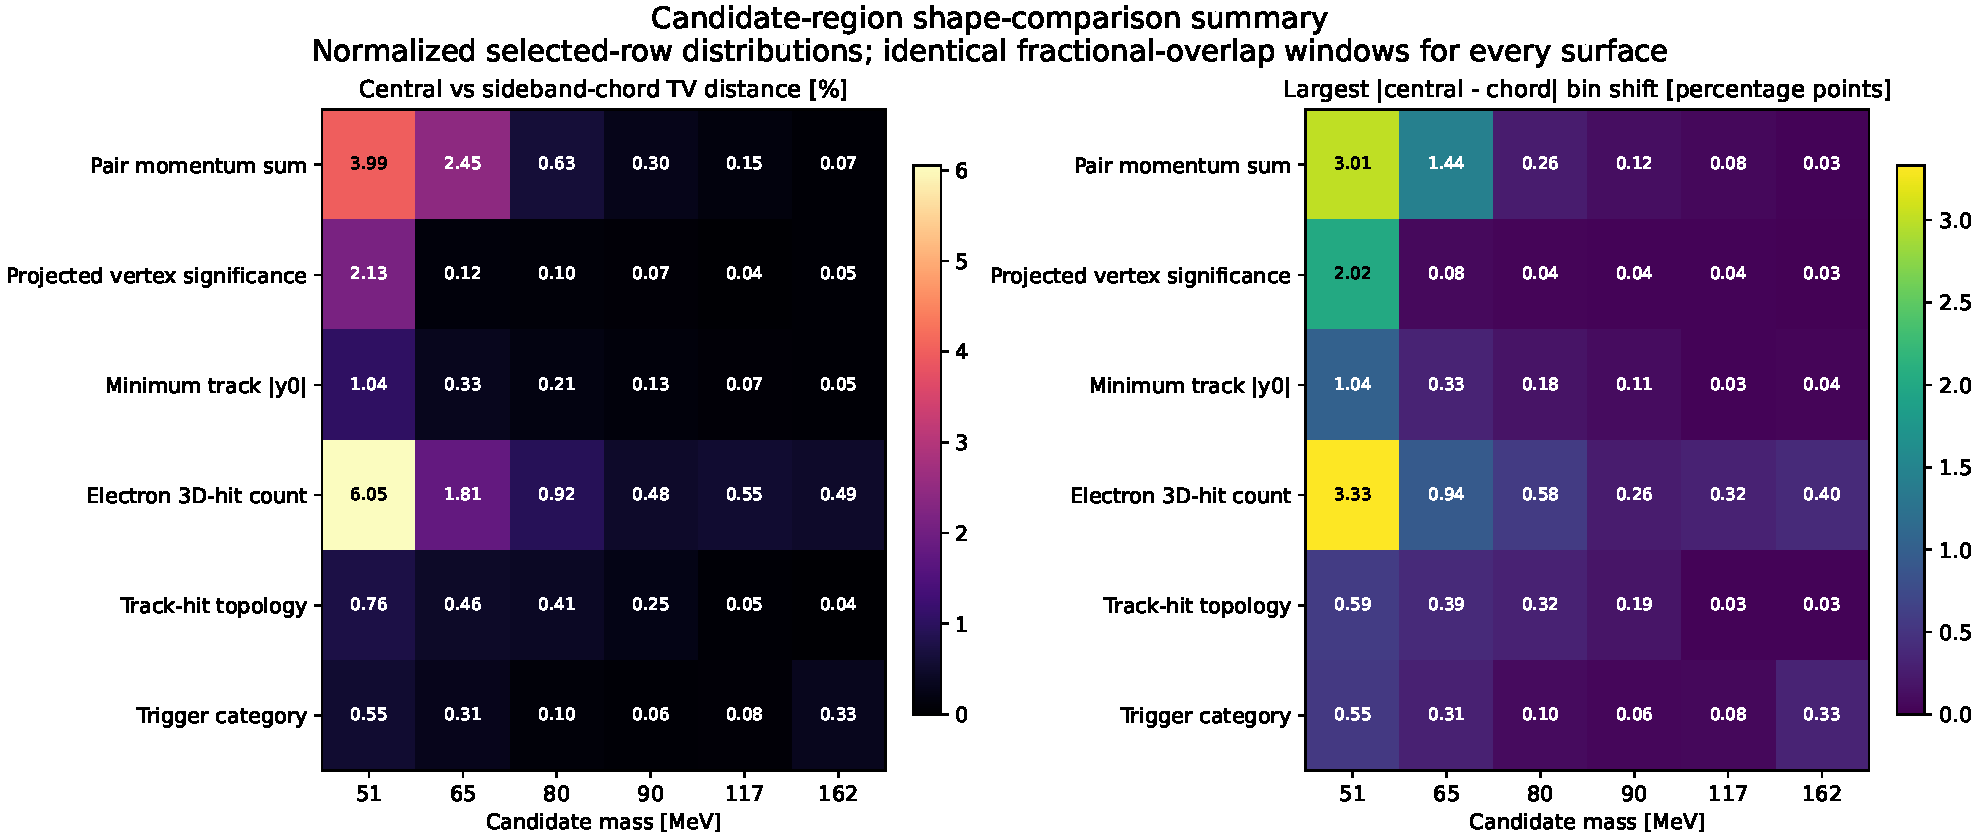
\includegraphics[width=0.98\linewidth]{final_limit_projection_figs/v4p3_candidate_region_variable_comparisons_20260811/candidate_region_tv_summary.pdf}
\caption{Total-variation distances between each overlap-weighted normalized
central-region distribution and the equal-sideband composition chord.  Values
are descriptive shape distances; they are not pulls, $p$-values, or
confidence intervals.}
\label{fig:v4p3-candidate-region-tv-summary}
\end{figure}

The summary in Figure~\ref{fig:v4p3-candidate-region-tv-summary} makes the
mass ordering quantitative.  At 51~MeV, the chord TV distances are 3.99\%
for momentum sum, 2.13\% for vertex-projection significance, 1.04\% for
minimum $|y_0|$, and 6.05\% for electron hit count; this is the strongest
left-to-right evolution and coincides with the lower-boundary/selection
turn-on region.  At 65~MeV the largest distances are 2.45\% in momentum sum
and 1.81\% in hit count, with 0.46\% in topology and 0.31\% in stored-trigger
composition.  The corresponding 80~MeV distances are smaller: 0.63\%,
0.92\%, 0.41\%, and 0.10\%, respectively.  The 90 and 117~MeV central shapes
closely interpolate their adjacent sidebands.  At 162~MeV the control and
topology distances remain small, with 0.49\% in hit count and 0.33\% in the
stored-trigger composition; this anchor is retained as a direct morphology
comparison beyond the current 40--160~MeV primary conditional-GPR domain.

The reciprocal 65/80 response reported by the frozen v4.2 inpainting/refit
is interpreted separately from these direct shape comparisons.  It is a
model-mediated response of the common nonlocal GP/background profile and can
be transmitted by the adjacent deficit/background structure.  The present
plots therefore retain 65 and 80~MeV as distinct local regions while avoiding
a physical-dependence interpretation.

The region comparisons keep both adjacent sidebands visible and use one
frozen grouping rule across anchors.  This supports like-for-like visual and
numerical comparisons while retaining ordinary mass evolution in the record.
Interpretation remains limited to the saved histogram axes and their
selected-row population; the plots do not supply an event-level signal
response or inferential calibration.

